
% Pro kompilaci po částech (viz projekt.tex), nutno odkomentovat a upravit
%\documentclass[../projekt.tex]{subfiles}
%\begin{document}

\chapter{Úvod}
TODO

\chapter{Přibližné výpočetní systémy} 
\label{acs}
S rostoucím využitím výpočetních technologií v mnoha různých oblastech lidské činnosti (v posledních letech zejména rapidní rozvoj strojového učení, zpracování velkých dat, aj.), rostou také nároky na výkon a efektivitu počítačů. Zároveň se zvyšují i nároky na mobilitu výpočetních systémů, mnoho zařízení obsahuje vestavěné systémy, což omezuje možnou velikost daných systémů.

Dle Moorova zákona se počet tranzistorů na jednom čipu každé 2 roky zhruba zdvojnásobí, ten ale pravděpodobně v dohledné době přestane vzhledem k fyzikálním vlastnostem tranzistorů platit \cite{moore}. Z tohoto důvodu je nutné se zamýšlet nad efektivnějším využitím výpočetních systémů.
Jedním z možných přístupů, který se v posledních letech těší velkému rozvoji jak ve výzkumu, tak v realné implementaci, je využití přibližných (aproximačních) výpočetních systémů.

V této kapitole bude nastíněn úvod do problematiky přibližných výpočetních systémů. Dále budou uvedeny oblasti, v nichž lze aproximaci použít a u kterých je naopak její použití nevhodné. Následuje přehled aproximačních technik, dále používaných hodnotících metrik a nakonec rozbor existujících přístupů k tvorbě aproximačních násobiček.

\section{Využitelnost a omezení přibližných výpočetních systémů}
Aproximační systémy lze typicky využít v oblastech, v nichž není nezbytně nutné znát přesný výsledek nějaké operace nebo výpočtu \cite{emerging_paradigm}. Takových oblastí je v informatice celá řada, zejména se jedná o zpracování multimédií, strojové učení, zpracování signálů, analýza velkých dat, webové vyhledávače, oblast rozšířené reality, počítačového vidění, aj. Využití aproximačních technik v některých zmíněných oblastech je popsáno níže.

\subsubsection{Zpracování signálů a obrazu}
V oblasti zpracování obrazu mohou přibližné výpočetní systémy zrychlit procesy jako je např. segmentace obrazu, tedy rozdělení obrazu do částí, které korespondují s konkrétními objekty v obraze (třeba pomocí aproximace algoritmů pro detekci hran) \cite{segmentation_tech}. Dále lze aproximaci využít při zlepšování kvality obrazu, např. při zvýraznění hran nebo při odstranění šumu.

\begin{figure}[H]
    \centering
    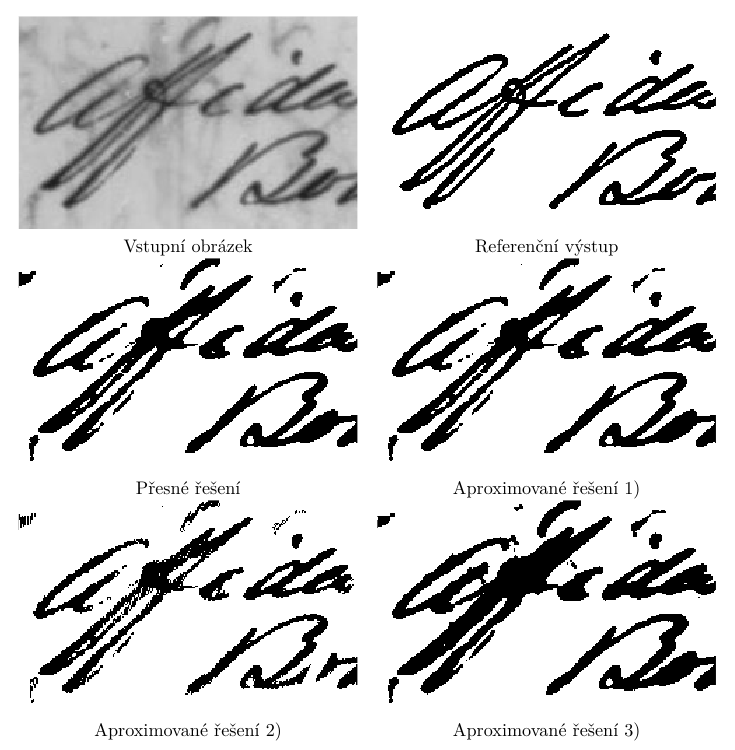
\includegraphics[width=0.9\textwidth]{obrazky-figures/approx_thresholding.png}
    \caption{Příklady výstupů aproximačních prahovacích algoritmů. Převzato z \cite{approx_image}}
    \label{fig:approx_threshold}
\end{figure}

\subsubsection{Analýza velkých dat}
Při zpracování tzv. velkých dat (angl. \textit{big data}) lze aproximovat dotazy na data, které jsou často velmi komplexní, výsledky jejich přibližných variant jsou ovšem mnohdy dostačující. Dále lze aproximovat i samotná data za účelem snížení nároků na úložný prostor. Pro nějakou třídu dotazů Q na data D musí platit, že pro aproximovaná data D' vrátí dotazy Q uspokojivé výsledky. Dotazy Q bývá obvykle potřeba mírně upravit, aby vyhovovala aproximovaným datům. V obou přístupech je třeba zvážit rovnováhu mezi efektivitou dotazů a kvalitou výsledků \cite{approx_big_data}.

\subsubsection{Strojové učení}
Přibližné počítání má ve strojovém učení (dále SU) obrovské využití, prostředí SU má totiž v mnoha ohledech ideální podmínky k využítí aproximace. Mnoho úloh SU lze redukovat na problém aproximace nějaké funkce, kde daná funkce není kompletně specifikována. Samotný proces trénování modelů lze přizpůsobit tak, aby se byl schopen zotavit ze všech případných nepříznivých účinků aproximace \cite{approx_ai}.

\begin{figure}[H]
    \centering
    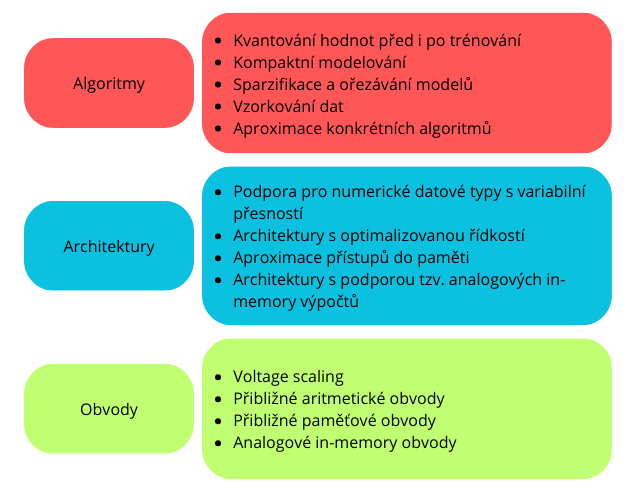
\includegraphics[width=0.7\textwidth]{obrazky-figures/ml.png}
    \caption{Přehled aproximačních technik používaných ve strojovém učení. Převzato z \cite{approx_ai}}
    \label{fig:enter-label}
\end{figure}

\subsubsection{Neaproximovatelné oblasti}
Přibližné výpočetní systémy naopak není vhodné využít tam, kde jsou z různých důvodů klíčové přesné výpočty. Typickým příkladem jsou jakékoliv peněžní transakce nebo algoritmy používané ve finančním inženýrství (angl. pojem \textit{Computational Finance}), kde by jakákoli nepřesná analýza mohla vést k velkým finančním ztrátám.

Dalším příkladem jsou tzv. bezpečnostně kritické systémy, v nichž by nepřesnosti mohly vést k ohrožení lidského života (např. systémy v automobilech, letadlech, elektrárnách, apod.).

Mezi nevhodné oblasti stran aproximace lze dále řadit třeba kryptografii a šifrování, high-precision manufaturing (vysoce přesná výroba), klasické databázové systémy, aj.

\section{Aproximační techniky}
V této sekci jsou stručně představeny některé používané aproximační techniky včetně uvedení jejich silných a slabých stránek a také konkrétních případů, kde je možné dané techniky využít \cite{ac_techniques}.

\subsection*{Precision scaling}
Škálování přesnosti je technika, při jejímž použití dochází ke snížení přesnosti aritmetických operací. Tuto techniku můžeme rozdělit na dva základní přístupy:
\begin{itemize}
    \item Statické škálování přesnosti -- Úroveň přesnosti je stanovena na jednu předem danou hodnotu pro všechny výpočty. Tato úroveň bývá určena na základě očekávané tolerance spouštěné aplikace vůči šumu. Hlavní výhodou tohoto přístupu je jeho jednoduchost. Nevýhodou je možná nízká efektivita stran úspory energie nebo zlepšení výkonu oproti dynamickému škálování.
    \item Dynamické škálování přesnosti -- Oproti statistickému škálování komplexnější technika, při níž je úroveň přesnosti výpočtů dynamicky stanovována na základě změn tolerance spouštěné aplikace vůči šumu za běhu. Snižuje tedy přesnost výpočtů v době, kdy je tolerance vůči šumu vysoká \cite{precision_scaling}.
\end{itemize}

Obecně je tedy škálování přesnosti vhodné pro aplikace, které zpracovávají velké množství dat, která zároveň obsahují velké množství šumu.

\subsection*{Loop perforation}
Perforace smyček se zaměřuje na zrychlení provádění smyček v programu pomocí odstranění některých iterací dané smyčky. Prvním krokem při používání této techniky bývá identifikace smyček, jejichž zkrácením či zjednodušením nedojde k výraznému zhoršení funkčnosti programu. K tomu lze využít specializovaný kompilátor, který na základě hranice zkreslení dané uživatelem tyto smyčky identifikuje a program následně upraví \cite{code_perforation}.

Tato technika má využití v oblastech numerických výpočtů, zpracování obrazu a signálu nebo v simulacích Monte Carlo.

\begin{verbatim}
    for( i = 0; i < h; i+=4 ) { 
        /* ... */ 
    }
\end{verbatim}

\begin{verbatim}
    for( i = 0; i < h; i+=4 ) {
        if (doPerforate(i, environment)) continue;
        //...
    }
\end{verbatim}

\subsection*{Load Value Approximation}
V případě, že se procesoru nepodaří načíst data z mezipaměti (anglicky tzv. \textit{cache load miss}), je procesor nucen přistoupit k vyšším úrovním mezipaměti nebo přímo do paměti, čímž vzniká větší latence. LVA využívá aproximovatelnost některých aplikací tím, že tato data odhaduje, takže procesor může dále běžet bez větších zpoždění \cite{ac_techniques}.

Příkladem využití může být technika použitelná u grafických aplikací, kdy load-value prediktor přistupuje do paměti pouze občas (narozdíl od klasických load-value prediktorů, které přistupují do paměti při každém load miss, aby ověřily správnost své predikce). Díky tomu se výrazně sníží počet přístupů do paměti, zatímco prediktor se přesto natrénuje kvalitně \cite{load_value_approx}.

\subsection*{Memoization}
Memoizace spočívá v ukládání výstupů funkcí za účelem jejich opětovného použití při volání funkcí se stejným vstupem. Tuto metodu lze dále aproximovat znovupoužíváním těchto výstupů i u funkcí s podobným vstupem. Dochází tedy ke zrychlení z důvodu menšího počtu výpočtů na úkor větší paměťové náročnosti.

Memoizace je nejlépe použitelná v aplikacích, v nichž se opakují často stejné vstupy, respektive výpočty. Příkladem mohou být různé rekurzivní algoritmy, např. výpočet Fibbonaciho posloupnosti, kombinatorické vzorce nebo vyhledávací algoritmy. Přibližnou variantu memoizace lze využívat v moderních grafických aplikacích, v nichž by standardní memoizace nepřinesla značné zrychlení \cite{ac_techniques}.

\subsection*{Inexact Hardware}
Využití nepřesného hardwaru (angl. \textit{inexact hardware}) spočívá v kontrolovaném zavádění chyb do výpočetních obvodů za účelem ušetření energie, zvýšení výkonu či zmenšení plochy obvodu. Toho lze docílit např. zjednodušováním aritmetických obvodů (k tomu více v podkapitole \ref{approx_mult}).

Na obrázku \ref{fig:approx_adder} je znázorněn příklad přibližné sčítačky využívající pouze OR hradla k sečtení nejméně významných bitů \cite{log_mults}.

\begin{figure}[H]
    \centering
    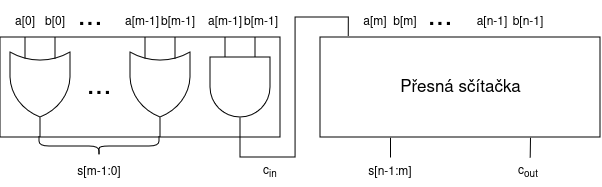
\includegraphics[width=\textwidth]{obrazky-figures/scitacka.png}
    \caption{Přibližná sčítačka lower-part-or s m nepřesnými bity. Převzato z \cite{log_mults}}
    \label{fig:approx_adder}
\end{figure}

\subsection*{Voltage Scaling}
Voltage Scaling (škálování napětí) je aproximační technika na úrovni obvodů. Jedná se o přístup, který umožňuje dynamicky měnit napětí dodávané do elektronických komponent, jako jsou mikroprocesory nebo grafické čipy, v závislosti na aktuálních požadavcích na výkon. Zvyšování napětí, tzv. \textbf{overvolting}, se používá pro zvýšení výkonu, \textbf{undervolting}, tedy snižování napětí, je využit při snaze ušetřit energii.

Při snižování napětí v obvodech mohou vznikat chyby. Například snižování napětí u paměti SRAM může vedle ušetření energie vést k častějším neúspěšným čtením a zápisům do paměti (\textit{read upset} a \textit{write failure}) \cite{ac_techniques}.

\pagebreak

\section{Hodnotící metriky}
Jednou z klíčových otázek při implementaci aproximačních systémů je vyhodnocení míry chybovosti těchto systémů. \textbf{Chybové metriky} porovnávají výsledky přesných systémů a jejich aproximačních variant z hlediska dané metriky. Seznam některých často používaných metrik je vypsán níže \cite{circuit_library} \cite{error_metrics}, symbol $n_i$ v rovnicích značí počet primárních vstupů, $O_{approx}$ a $O_{orig}$ značí výstupy přibližných, respektive přesných systémů.

\bigskip

\textbf{Hammingova vzdálenost} (angl. Hamming distance, zkr. HD) mezi dvěma bitovými sekvencemi je rovna počtu pozic, na kterých se bity obou sekvencí liší \cite{hamming_dist}. Mezi používané varianty této metriky patří \textit{Průměrná Hammingova vzdálenost} nebo \textit{Maximální Hammingova vzdálenost} (v angličtině se používá výraz \textit{bit-flip error}).

Pro posuzování chybovosti násobiček není tato metoda příliš vhodná. Pokud je například očekávaný přesný výsledek výpočtu $64_{10} = 0100 0000_{2}$ a výsledek aproximace $63_{10} = 0011 1111_{2}$, jejich Hammingova vzdálenost je 7, zatímco relativní chyba je cca. $1,5 \%$.
\begin{equation}
    HD = \sum_{\forall i} OnesCount(O_{approx}^{(i)} \oplus O_{orig}^{(i)})
\end{equation}

\textbf{Pravděpodobnost chyby} (angl. error probability, zkr. EP) značí, s jakou pravděpodobností nebude výstup aproximačního systému odpovídat výstupu přesného systému.
\begin{equation}
    EP = \frac{\sum_{\forall {i:O_{approx}^{(i)} \neq O_{orig}^{(i)}}} 1} {2^{n_i}}
\end{equation}

\textbf{Průměrná absolutní chyba} (angl. mean absolute error, zkr. MAE) popisuje průměrný rozdíl mezi přesnými a přibližnými výstupy.
\begin{equation}
    MAE = \frac{\sum_{\forall i} {\left|{{O_{approx}^{(i)} - O_{orig}^{(i)}}}\right|}} {2^{n_i}}
\end{equation}

\textbf{Průměrná kvadratická chyba} (angl. mean squared error, zkr. MSE) počítá průměr druhých mocnin rozdílů mezi přesnými a přibližnými výstupy. MSE se často používá při výpočtu tzv. PSNR (zkratka z anglického \textit{Peak signal-to-noise ratio}, česky \textit{Špičkový poměr signálu k šumu}), pomocí kterého lze určovat kvalitu rekonstrukce obrázků a videí \cite{error_metrics}.
\begin{equation}
    MSE = \frac{\sum_{\forall i} {\left|{{O_{approx}^{(i)} - O_{orig}^{(i)}}}\right|^2}} {2^{n_i}}
\end{equation}

\textbf{Průměrná relativní chyba} (angl. mean relative error, zkr. MRE) uvažuje průměrnou chybu v relaci s velikostí očekávaného výstupu. Díky tomu jsou při větších hodnotách akceptovatelné větší chyby.
\begin{equation}
    MRE = \frac{\sum_{\forall i} \frac{\left|{{O_{approx}^{(i)} - O_{orig}^{(i)}}}\right|} {max(1,O_{orig}^{(i)})}} {2^{n_i}}
\end{equation}

\textbf{Nejhorší absolutní chyba} (angl. worst-case error, zkr. WCE) popisuje největší možnou chybu, které je možné při aproximaci dosáhnout.
\begin{equation}
    WCE = \max_{\forall i} \left|{O_{approx}^{(i)} - O_{orig}^{(i)}}\right|
\end{equation}

\textbf{Nejhorší relativní chyba} (angl. worst-case relative error, WCRE) uvažuje největší možnou chybu aproximačního výstupu vzhledem k očekávanému výstupu.
\begin{equation}
    WCRE = \max_{\forall i} \frac{\left|{O_{approx}^{(i)} - O_{orig}^{(i)}}\right|} {\max(1,O_{orig}^{(i)})} 
\end{equation}

\bigskip

U aproximačních obvodů jsou neméně důležité jejich \textbf{fyzické vlastnosti}. Mezi základní z nich lze zařadit zpoždění, příkon a plochu obvodu. Tyto vlastnosti je možné kombinovat v různé další složené metriky, např. PDP (z angl. \textit{Power-delay product}, tedy součin ztrát výkonu a zpoždění obvodu), ADP (z angl. \textit{Area-delay product}, tedy součin plochy a zpoždění obvodu) nebo EDP (z angl. \textit{Energy-delay product}, tedy součin zpoždění a spotřebované energie obvodu) \cite{approx_arith_circuits}.

\bigskip

Aproximační systémy je dále možné posuzovat vhodnými \textbf{kvalitativními metrikami} vzhledem k využití daného systému v konkrétní aplikaci. Mezi často používané metriky \cite{ac_techniques} patří např. výše zmíněné \textbf{PSNR}, \textbf{SSIM} (zkratka z angl. \textit{Structular similarity}, česky tedy \textit{strukturální podobnost}), \textbf{Rozdíl pixelů} (angl. \textit{Pixel difference}) nebo \textbf{UIQI} (zkratka z angl. \textit{Universal Image Quality Index}, česky tedy \textit{Univerzální index kvality obrazu}), které se používají při porovnávání podobnosti obrázků a videí.

Výstupy systémů založených na strojovém učení nebo na shlukování lze posuzovat např. na základě \textbf{Přesnosti} (angl. \textit{Precision}), \textbf{Výtěžnosti} (angl. \textit{Recall}), metrikou \textbf{F-score}, nebo dalších složitějších metrik \cite{clustering_eval}.

\section{Aproximační násobičky} \label{approx_mult}
Násobení je operace, která je při spouštění datově náročných aplikací (např. streamování, zpracování obrazu, strojové učení, aj.) utilizována velmi často a která tím pádem spotřebuje nemalé množství energie. Mnohé z těchto aplikací jsou ovšem schopné vytvořit dostatečně dobrý výsledek i přes nepřesnosti v násobení. Dalším příkladem využití přibližných násobiček jsou zařízení z oblasti internetu věcí, u nichž je kladen důraz na co nejmenší spotřebu energie a u nichž také mnohdy není nutné vše počítat přesně \cite{approx_mult_survey}. 

Tato podkapitola se zaměřuje nejprve na vysvětlení funkcionality binárních násobiček a následně na popis základních přístupů k vytváření přibližných násobiček.

\subsubsection{Základní princip binárních násobiček}
Při binárním násobení uvažujeme pouze 2 hodnoty -- 1 a 0, z toho důvodu je možné na binární násobení nahlížet jako na sekvenci sčítání a bitových posunů. Uvažme příklad z obrázku \ref{fig:binmult}, kde vstup $x$ je násoben vstupem $y$. Operaci násobení lze rozdělit do 3 fází: načtení dat na vstupu, generování částečných součinů a finální suma.

Základní binární násobička funguje tak, že se postupně roznásobují jednotlivé bity vstupu $y$ se všemi bity vstupu $x$ a následně na základě váhy bitu $y$ dochází k bitovému posunu vlevo. První řádek částečných součinů v příkladu z obrázku \ref{fig:binmult} tedy vznikne roznásobením bitu $y_0$ se všemi bity vstupu $x$, atd. Nakonec se všechny částečné 1součiny sečtou v konečný výsledek.

\begin{figure}[H]
    \centering
    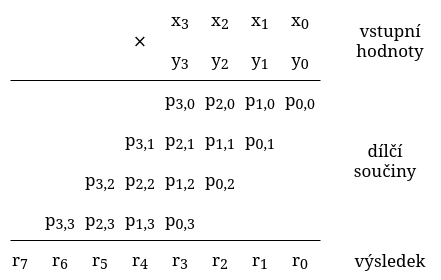
\includegraphics[width=0.55\textwidth]{obrazky-figures/binmult.png}
    \caption{Binární násobička 4x4 bity}
    \label{fig:binmult}
\end{figure}

Násobení jednotlivých bitů je implementováno jednoduše pomocí hradel AND, kritickou sekcí procesu násobení je propagace přenosu (angl. \textit{carry}) z nižšího bitu na vyšší bit. Přístupů k řešení tohoto problému je mnoho, jedním z nich je například tzv. ripple-carry sčítačka, kde se přenosy propagují postupně zprava doleva, nebo také tzv. carry-save sčítačka, kde se přenosy propagují diagonálně za účelem zrychlení výpočtu \cite{approx_mult_survey}.

\begin{figure}[H]
    \centering
    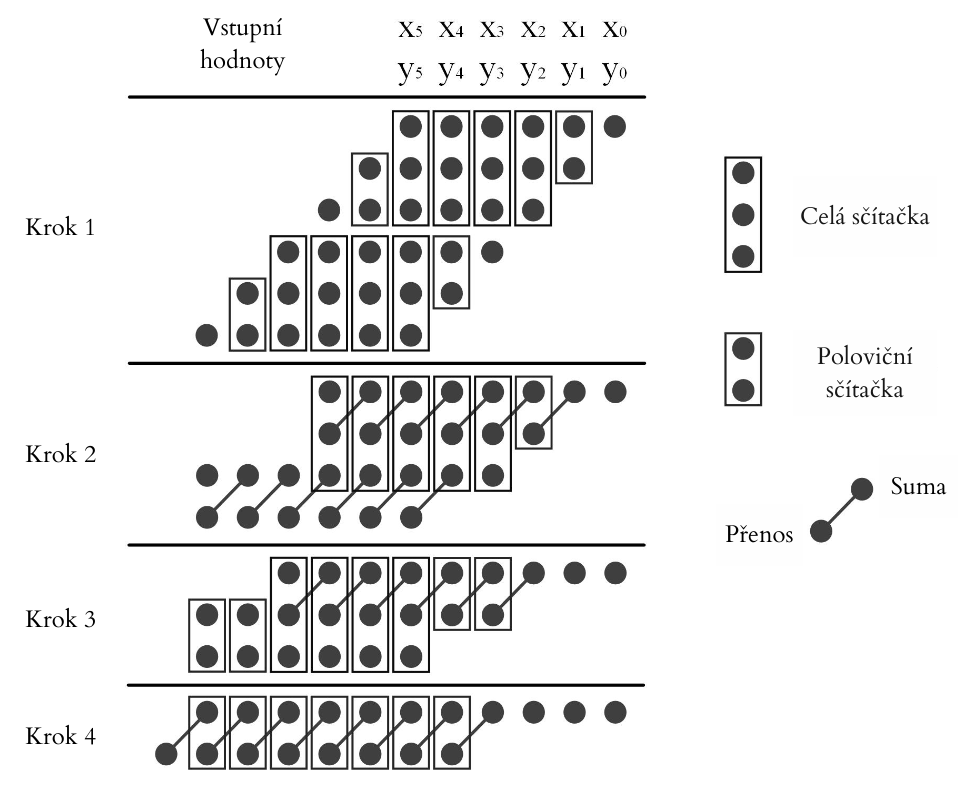
\includegraphics[width=0.75\textwidth]{obrazky-figures/wallacetree.png}
    \caption{Příklad Wallace-Tree násobičky. Převzato z \cite{approx_mult_survey}}
    \label{fig:wallacetree}
\end{figure}

Další zrychlení přináší princip tzv. Wallace Tree, v rámci něhož se seskupují 3 částečné součiny po sloupcích, které generují 2 výstupy -- sumu a přenos. Tato operace se opakuje, dokud nezůstanou poslední dva řádky částečných součinů, které se poté sečtou v konečný výsledek. V této násobičce jsou využívány úplné a částečné sčítačky, dalšího zrychlení lze docílit utilizací paralelních výpočtů \cite{wallace_tree}. Ilustrace této násobičky je na obrázku \ref{fig:wallacetree}.

\subsubsection{Aproximace vstupních hodnot}
Jednoduchým a přesto efektivním způsobem aproximace je aproximace vstupních dat. Toho lze docílit např. uříznutím několika nejméně významných bitů (zkr. LSB z angl. \textit{least significant bit}), což má menší vliv na celkový výsledek výpočtu, než uříznutí několika nejvíce významných bitů (zkr. MSB z angl. \textit{most significant bit}) \cite{approx_mult_survey}. 

Existují dvě základní metody segmentace dat -- dynamická a statická. Dynamická segmentace dat (DSM) spočívá v detekci prvního nenulového bitu a oříznutí následujících $k$ bitů. Při statické segmentaci dat (SSM) dochází k volbě jedné z předem daných strategií. Na obrázku \ref{fig:dsm_ssm} jsou ilustrovány obě metody, u SSM jsou v tomto případě následující možnosti: $k$ nejméně významných bitů, $k$ nejvíce významných bitů nebo $k$ prostředních bitů jako kompromis.

SSM zpravidla potřebuje méně hardwarových zdrojů než DSM, na druhou stranu její výsledek bývá méně efektivní, protože může obsahovat některé redundantní bity (např. nulové MSB).

\begin{figure}[H]
    \centering
    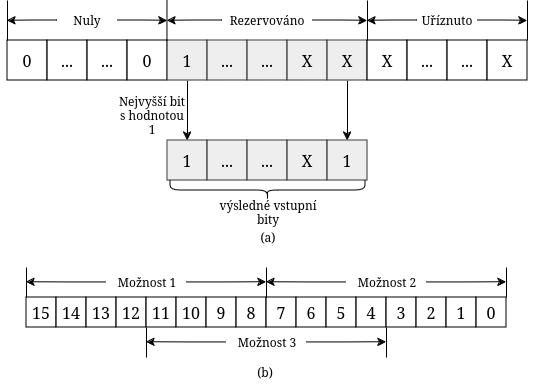
\includegraphics[width=0.8\textwidth]{obrazky-figures/dsm_ssm.png}
    \caption{(a) Příklad oříznutí DSM; (b) Příklad oříznutí SSM. Převzato z \cite{approx_mult_survey}}
    \label{fig:dsm_ssm}
\end{figure}

\subsubsection{Aproximace při generování částečných součinů}
Jedním z možných přístupů je využití malých bloků nepřesných násobiček k vytvoření dílčích součinů a poté sečtení těchto různě bitově posunutých dílčích součinů. Takové násobičky lze nazývat pojmem \textit{Nedostatečně navržená násobička} neboli anglicky \textbf{Under-designed multiplier}. 

Příkladem stavebního bloku může být násobička na obrázku TODO. Jak lze pozorovat v Karnaughově mapě v tabulce \ref{tab:kmap2x2}, tato násobička je přesná pro 15 ze 16 možných vstupních kombinací (nepřesný výsledek je v tabulce vyznačen červeně). Změna oproti přesné násobičce je v tom, že výsledek vstupu $3*3$ je reprezentován bity $111$ oproti přesnému výsledku $1001$, díky čemuž se snížila plocha obvodu téměř na polovinu (5 logických hradel oproti 9 u přesné násobičky, méně drátů) s pravděpodobností chyby pouze $\frac{1}{16}$ \cite{underdesigned_mult}.

\begin{table}[H]
\centering
\begin{tabular}{|
>{\columncolor[HTML]{FFFFFF}}l |
>{\columncolor[HTML]{FFFFFF}}l |
>{\columncolor[HTML]{FFFFFF}}l |
>{\columncolor[HTML]{FFFFFF}}l |
>{\columncolor[HTML]{FFFFFF}}l |}
\hline
 $*$  & 00  & 01  & 11                         & 10  \\ \hline
00 & 000 & 000 & 000                        & 000 \\ \hline
01 & 000 & 001 & 011                        & 010 \\ \hline
11 & 000 & 011 & {\color[HTML]{FE0000} 111} & 110 \\ \hline
10 & 000 & 010 & 110                        & 100 \\ \hline
\end{tabular}
\caption{Karnaughova mapa pro nepřesnou násobičku z obrázku TODO}
\label{tab:kmap2x2}
\end{table}

Na obrázku \ref{fig:larger_mults} je znázorněn příklad násobičky 4x4 bitů složené ze 4 bloků násobiček 2x2
bity. A a X jsou vstupní hodnoty, dolní indexy H, respektive L značí 2 vyšší, respektive 2 nižší bity vstupu. V jednotlivých blocích postupně dochází k roznásobení všech kombinací dvojich vstupních bitů, tyto dílčí výsledky jsou následně bitově posunuty a sečteny, čímž vzniká celkový výsledek násobení.

\begin{figure}[H]
    \centering
    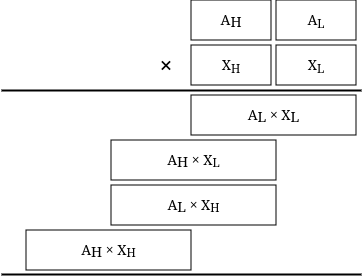
\includegraphics[width=0.6\textwidth]{obrazky-figures/larger_mults.png}
    \caption{Tvorba násobiček z menších bloků. Převzato z \cite{underdesigned_mult}}
    \label{fig:larger_mults}
\end{figure}

\subsubsection{Aproximace při finálním sčítání}


\chapter{Statistické ověřování modelů}
\label{smc}
TODO

\chapter{Rozbor a návrh řešení}
\label{rozbor}
TODO

\chapter{Popis řešení}
\label{popis}
TODO

\chapter{Zhodnocení výsledků} 
\label{zhodnoceni}
TODO

\chapter{Závěr}
\label{zaver}
TODO

%===============================================================================

% Pro kompilaci po částech (viz projekt.tex) nutno odkomentovat
%\end{document}

